\documentclass[11.5pt]{sig-alternate}
\usepackage{hyperref}
\usepackage{tabularx}
\usepackage{graphicx}
\usepackage{blindtext}
\usepackage[utf8]{inputenc}
\usepackage[english]{babel}
\usepackage{lastpage}
\usepackage{comment}
\usepackage{dirtytalk}
\usepackage{xcolor}
\usepackage{hanging}
\usepackage{wrapfig}
\usepackage[backend=biber,style=apa]{biblatex}
\addbibresource{notation.bib}
\usepackage{authblk}
\usepackage{caption}
\usepackage{longtable}
\usepackage{graphicx,subfigure}
\usepackage{authblk}
\usepackage{enumitem}
\usepackage[utf8]{inputenc}
\usepackage{cuted}
\usepackage{fancyhdr}
\pagestyle{fancy}
\usepackage{lipsum}
\renewcommand{\headrulewidth}{0pt}
\renewcommand{\footrulewidth}{0pt}
\setlength\headheight{80.0pt}
\addtolength{\textheight}{-80.0pt}
\usepackage{amssymb}
\setcounter{tocdepth}{2}
\chead{%
  \ifcase\value{page}
  % empty test for page = 0
  \or 
\includegraphics[width=\textwidth]{headerImage.png}% page = 1
  \or 
\includegraphics[width=\textwidth]{headerImage.png}% page = 2
  \or 
\includegraphics[width=\textwidth]{headerImage.png}% page = 3
  \or 
\includegraphics[width=\textwidth]{headerImage.png}% page = 4
  \or 
\includegraphics[width=\textwidth]{headerImage.png}% page = 5
  \else
  
\includegraphics[width=\textwidth]{headerImage.png}
  \fi
}
%\chead{
\includegraphics[width=\textwidth]{headerImage.png}}
\fancyfoot[LE,LO]{Universal Design for Learning (UDL) in Inclusive  Preschool Science Classrooms\\           
DOI: 10.14448/jsesd.14.0006}
\fancyfoot[CE,CO]{{ }}
\fancyfoot[RE,RO]{\thepage}
\pagenumbering{arabic}
\hypersetup{
    colorlinks=true,
    urlcolor=blue
}
 
\let\oldabstract\abstract
\let\oldendabstract\endabstract
\makeatletter
\renewenvironment{abstract}
{\renewenvironment{quotation}%
               {\list{}{\addtolength{\leftmargin}{1em} % change this value to add or remove length to the the default
                        \listparindent 1.5em%
                        \itemindent    \listparindent%
                        \rightmargin   \leftmargin%
                        \parsep        \z@ \@plus\p@}%
                \item\relax}%
               {\endlist}%
\oldabstract}
{\oldendabstract}
\makeatother

% Left align captions
\captionsetup{justification   = raggedright,
              singlelinecheck = false}
       
    \begin{document}


\title{Universal Design for Learning (UDL) in Inclusive \\Preschool Science Classrooms}

\author[1]{\large \color{blue} Marla J. Lohmann}
\author[2]{\large \color{blue} Katrina A. Hovey}
\author[3]{\large \color{blue}   Ariane N. Gauvreau}


\affil[1]{Colorado Christian University}
\affil[2]{Western Oregon University}
\affil[3]{Western Oregon University}
\toappear{}

\maketitle

%% ABSTRACT

\begin{@twocolumnfalse} 

\begin{abstract}
\item 
     \textit{Science instruction is a critical aspect of early learning. Teachers can support young children’s learning about scientific concepts through the use of the Universal Design for Learning (UDL) framework, which is a proactive approach to instructional planning that helps ensure success for all learners. 
     This teaching techniques article offers preschool teachers practical solutions for implementing in the UDL framework for science instruction in their classrooms.}
     \\
     \\
     Keywords: early childhood, preschool, science, universal design for learning\\
\end{abstract}

\end{@twocolumnfalse}
%% AUTHOR INFORMATION

\textbf{*Corresponding Author, Marla J. Lohmann} \\
\href{mailto:mlohmann@ccu.edu}{(mlohmann@ccu.edu)} \\
\textit{Submitted October 03, 2021 }\\
\textit{Accepted July 09, 2022} \\
\textit{Published online November 21, 2022} \\
\textit{DOI: 10.14448/jsesd.14.0006} \\
\pagebreak
\pagebreak

\vspace{5mm}
\section*{\vspace{140mm}}
\section*{Universal Design for Learning (UDL) in Inclusive Preschool Science Classrooms}
\begin{large}

\emph {Ms. Rosa teaches in an inclusive pre-kinder-garten classroom and is currently teaching a unit on insects. Ms. Rosa wants to ensure that she captures the interest of all learners in her classroom and that she presents the concepts in a manner that leads to young children learning. In order to achieve this, she is using the Universal Design for Learning framework as she designs the instructional activities for this learning unit.}

Science instruction is vital in the early childhood classroom and about a quarter of instructional time in the preschool classroom is spent on science-related tasks (Piasta et al., 2014) such as observing the world around them and solving problems (Dilek et al., 2020). The National Science Teaching Association (NSTA; 
\\2014) published a position statement that supports the importance of teaching young children scientific concepts; common preschool science concepts include the human body, living and nonliving things, physical attributes of objects, and space (Guo et al., 2015). In the NSTA statement, they assert that young children can learn about the world around them through a variety of formal and informal instruction that focuses on providing opportunities for experiential learning. In this article, we offer practical suggestions for supporting young children in learning science concepts through the use of the Universal Design for Learning (UDL) framework.

\section*{Universal Design for Learning}

Universal Design for Learning is a framework for developing instruction in the classroom \\through intentional and proactive planning for diverse learning needs and preferences (CAST, 2018). UDL includes three principles that work together to support children’s learning: (a) multiple means of engagement, (b) multiple means of representation, and (c) multiple means of action and expression (CAST, 2018; Rose \& Strangman, 2007). Each of the three principles includes checkpoints that specifically target learners’ ability to (a) access, (b) build, and (c) internalize the information they are learning (CAST, 2018).

The Division for Early Childhood has outlined Recommended Practices that represent high quality, evidence-based instruction in the inclusive early childhood classroom. UDL is aligned with four of the practices; specifically E1, E2, INS1, and INS5 (DEC, 2014):
\begin{quote} E1. Practitioners provide services and supports in natural and inclusive environments
during daily routines and activities to promote the child’s access to and
participation in learning experiences.
\\E2. Practitioners consider Universal Design for Learning principles to create accessible
environments.
\\INS1. Practitioners, with the family, identify each child's strengths, preferences, and
interests to engage the child in active learning.
\\ INS5. Practitioners embed instruction within and across routines, activities, and
environments to provide contextually relevant learning opportunities.\end{quote} 
In addition to the DEC Recommended Practices, the use of UDL also aligns with the DEC Early Interventionist/Early Childhood Special Educator (EI/ECSE) Standard 5: Application of curriculum frameworks in the planning of meaningful learning experience (DEC, 2020). Through the use of UDL, preschool teachers can ensure that the curriculum is aligned with the needs of all learners, which can reduce the need for some individualized interventions (CAST, 2006).

The UDL framework has been shown effective for meeting the needs of young children in the inclusive classroom (Chen \& Dote-Kwan, 2021; Parette \& Blum, 2014; Stockall et al., 2012). The UDL framework supports learning for various early childhood developmental skills and routines including circle time (Gauvreau et al., 2021), science, technology, engineering, and mathematics (STEM) instruction (Gonzalez \& Fryer, 2014), mathematics (Selmer \& Floyd, 2012), and gross motor development (Taunton et al., 2017). In addition, the use of the UDL framework paired with other effective teaching practices such as Multi-Tiered Systems of Support (MTSS; see https://mtss4success.org) and embedded learning, can promote inclusion in the early childhood classroom (Coogle et al., 2022).

This article presents early childhood teachers with practical ideas for implementing the three UDL principles during preschool science instruction. Table 1 outlines specific teaching practices that can be used to meet each principle, but teachers should keep in mind that this list is not exhaustive and that instruction designed using the UDL framework will look different in each classroom.

\section*{Table 1}
  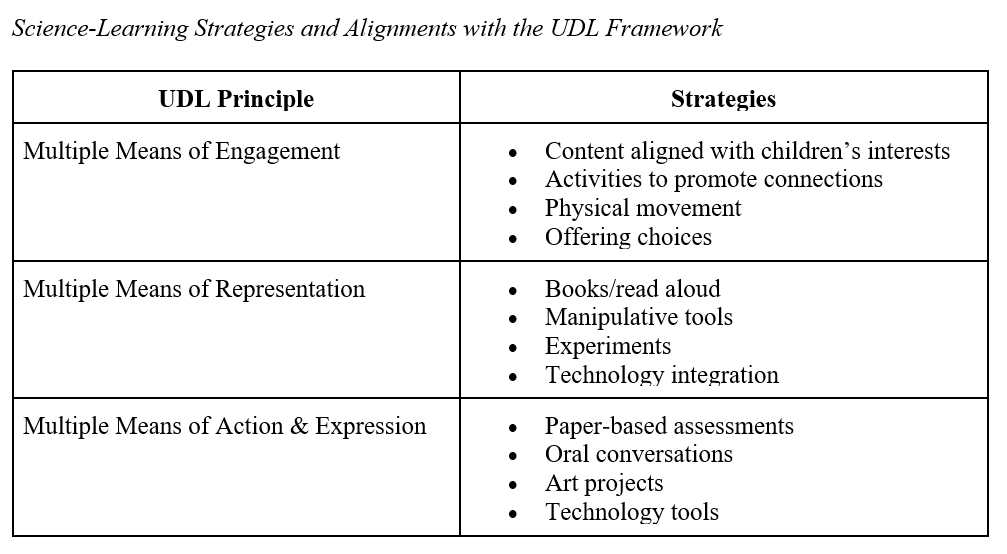
\includegraphics[width=8cm]{Table 1.png}
    \label{Science-Learning Strategies and Alignments with the UDL Framework}   

\section*{Multiple Means of Engagement}
The first UDL principle is multiple means of engagement, which targets the affective brain network (Glass et al., 2013) and includes the teaching strategies used to engage and motivate learners (Lohmann et al., 2018). Early childhood teachers can meet this principle in a variety of ways during science instruction, with a few ideas being: (a) including content that aligns with children’s interests, (b) the use of learning activities that promote connections in learning, (c) incorporating physical movement in learning, and (d) offering choices in learning.
\\\\
\textbf{\emph Content Aligned with Children’s Interests}\\\\
Young children are frequently more motivated to engage in learning when that learning includes materials aligned with their interests (Sandall et al., 2019). Aligning instruction to young children’s interests is a key feature of differentiated learning (Tomlinson et al., 2003) and foundational to culturally responsive practice (Gay, 2010; Ladson-Billings, 2014). Research demonstrates that aligning learning with children’s interests increases their motivation, focus, engagement, and achievement (Harackiewicz et al., 2016). Preschool teachers can select science units that align with children’s interests, such as a unit study on bugs when the children show interest in the ants on the playground. Additionally, children’s interests can be incorporated into already existing science units. For example, while learning about water buoyancy, young children can test to see if their favorite toys or classroom learning tools float or sink.  
\newpage
\textbf{\emph Activities to Promote Connections}

Best practice in early childhood education involves children’s active participation in the learning community. Effective instruction for learners of all ages involves positive interaction between learners and the teacher (Rhoad-Drogalis et al., 2018) and between learners and other learners (Veziroglu-Celik \& Acar, 2020). Teacher-child relationships have long-term impacts on children’s outcomes in all areas (Ansari et al., 2020); teachers can support these relationships by getting to know each child as a unique learner and spending one-on-one time with children during science lessons. Science centers and other independent or small-group tasks provide an ideal time for teachers to dedicate to this individualized time.

In order to promote connections between learners, teachers should intentionally design some science learning activities to be completed with peers and must systematically teach young children how to work together to complete their learning tasks (Alanis, 2018). Science activities such as experiments are the ideal learning opportunities for collaborative work. The authors recommend, though, that early childhood educators explicitly teach young children how to work with others before assigning them to complete science activities with partners or small groups. Table 2 provides a list of critical collaboration skills for young children and ways in which we might see young children exhibit these skills during Science instruction.

\section*{Table 2:\textit{Collaboration Skills in Preschool}}

\noindent\begin{minipage}{\linewidth}
\centering
\resizebox{\linewidth}{!}{%
\begin{tabular}{|l|l|} 
\hline
Skill & Example \\ 
\hline
\begin{tabular}[c]{@{}l@{}}Sharing toys and \\learning materials\end{tabular} & \begin{tabular}[c]{@{}l@{}}The children are \\planting a garden, \\but there are not \\enough shovels \\for each child \\to have their own. \\When the children \\ are done using the \\shovel, they give it \\to a classmate.\end{tabular} \\ 
\hline
Taking turns & \begin{tabular}[c]{@{}l@{}}Leo and Sarai are \\both painting \\pictures of the class \\fish. The fish is blue, \\but there is only one\\container of blue paint, \\ so the children take \\turns putting their \\paint brushes into \\ the paint jar.\end{tabular} \\ 
\hline
\begin{tabular}[c]{@{}l@{}}Listening when others \\are speaking\end{tabular} & \begin{tabular}[c]{@{}l@{}}Azami is sharing with \\the class her \\hypothesis about what \\ will happen to the ice \\cube that is sitting in \\the windowsill. \\ While she speaks, \\her classmates look \\at her and listen to \\ what she is saying.\end{tabular} \\ 
\hline
\begin{tabular}[c]{@{}l@{}}Responding appropriately to \\statements made by others\end{tabular} & \begin{tabular}[c]{@{}l@{}}After Azami finishes \\sharing her hypothesis, \\Kamal builds upon what \\she said by telling a story\\about ice melting in his juice \\glass during the summer.\end{tabular} \\ 
\hline
\begin{tabular}[c]{@{}l@{}}Responding appropriately \\when frustrated with a peer\end{tabular} & \begin{tabular}[c]{@{}l@{}}Matthew is using the \\magnifying glass to look \\at insects in the class \\garden. Joey walks over, \\takes the magnifying \\ glass from Matthew, \\and uses it. Matthew \\feels angry, but \\ chooses to take a \\deep breath before \\calmly asking Joey \\ to return the magnifying glass.\end{tabular} \\ 
\hline
\begin{tabular}[c]{@{}l@{}}Sharing responsibility for \\completing a task\end{tabular} & \begin{tabular}[c]{@{}l@{}}After the Science lesson \\is over, Mr. Manuel \\instructs the children to \\clean up their work \\spaces. Laila and Nia \\ work together to carry \\the sensory tub to the \\sink and then dump it.\end{tabular} \\
\hline
\end{tabular}
}
\end{minipage}\\\\
\textbf{\emph Physical Movement}\\\\
There is a direct correlation between physical activity and learning (deWaal, 2019). Young children learn content better and are more motivated to learn when they are moving (Furmanek, 2014; Mavilidi et al., 2018). Movement can be incorporated into science instruction in various ways including activities such as (a) nature walks, (b) acting out scientific processes, such as life cycles, (c) marching around the room while the class chorally shouts information, (d) walking like various animals, and (e) playing games related to science concepts on the playground.\\\\
\textbf{\emph Offering Choices }\\\\
All learners appreciate having choices in their daily learning experiences (McInnis et al., 2011); for young children, this is especially true when that learning involves play in the classroom or other settings (King \& Howard, 2014). The use of choice in learning can support young children’s self-determination skills and autonomy (Jolivette et al., 2002), as well as decrease challenging behaviors in the classroom (Blair et al., 2010) and increase time-on-task for young children (Wiltz \& Klein, 2001). Preschool teachers can offer choice in a variety of ways during science instruction. Young children may be offered a variety of options, such as (a) where to sit during instruction, (b) whether to complete experiments and other hands-on learning alone or with a partner, (c) completing work using pencil/paper or technology tools, and (d) which assessment format to complete to demonstrate their learning.  
Ms. Rosa wants to focus on multiple means of engagement as she designs her lessons for the week. She plans a nature walk around the school to look for insects, reflecting on how her class loves to explore outdoors, and organizes children into pairs and trios so they can work together. She plans opportunities for children to plan how they would like to search for insects - under rocks or logs, in the flower bed, around the trees that line the playground, etc. - at circle time before they leave, and supports each group to create a plan using pictures of areas they would like to search (e.g, the flower bed, under rocks, etc.). This will enable children to collaborate and have the autonomy to make their own choices during the activity. The visuals will also help specific children remain on task, and support choice making in the moment. During the nature walk, she observes children taking turns carrying their clipboard and visual plans, happily exploring and locating many different insects around the school property. Ms. Rosa takes photos of the insects they find on her smartphone, and plans to print these out so they can discuss them at afternoon circle. She is thrilled with how simple embedded Multiple Means of Engagement was in this activity, and notices how captivated children were during the nature walk! 
\section*{Multiple Means of Representation}

The UDL principle of multiple means of representation is aligned with the recognition brain network (Glass et al., 2013) and focuses on the various ways in which early childhood teachers present instruction in the classroom (Gauvreau et al., 2019). In preschool science instruction, teachers can use strategies such as (a) books, (b) experiments, (c) puzzles and other manipulative tools, and (d) technology integration to meet this principle.
\newpage
\textbf{\emph Books and Read-Alouds}

Reading to young children is a vital part of early learning (Alatalo \& Westlund, 2021) and early childhood teachers often include read-alouds paired with discussion as an instructional method (Ezell \& Justice, 2005). When teaching science concepts, teachers can, and should, incorporate fiction and non-fiction books related to the topic. In addition to hearing the teacher read the books, young children can also explore the books on their own in the Library Center and listen to an audio version of the book in the Listening Center. Table 3 offers a short, but not comprehensive, list of preschool-friendly nonfiction books about science topics. 
% Please add the following required packages to your document preamble:
% \usepackage{graphicx}
\section*{Table 3}
\textit{Books for Preschool Science Lessons}\\\\
\noindent\begin{minipage}{\linewidth}
\resizebox{\columnwidth}{!}{%

\begin{tabular}{|l|l|}
\hline
\textbf{Book Title and Author}  & \textbf{Topic} \\ \hline

\begin{tabular}[c]{@{}l@{}}\textit{What is Science?}\\    \\ By: Rebecca Kai Dotlich\end{tabular}  & \begin{tabular}[c]{@{}l@{}}This book  presents the subject of \\ science and scientific inquiry and \\ is ideal for use at the beginning of \\ the school year in order to launch \\ science learning.\end{tabular} \\ \hline

\begin{tabular}[c]{@{}l@{}}\textit{I use Science Tools}\\    \\ By: Kelli Hicks\end{tabular}  & \begin{tabular}[c]{@{}l@{}}This book can be used to help young \\ children learn about the tools, such \\ as magnifying   glasses, they will \\ use to learn scientific concepts in \\ the classroom.\end{tabular}  \\ \hline

\begin{tabular}[c]{@{}l@{}}\textit{Floating and  Sinking}\\    \\ By: Amy S. Hansen\end{tabular} & \begin{tabular}[c]{@{}l@{}}This book can be  used at the \\ beginning of a unit on the properties \\ of water.\end{tabular}  \\ \hline

\begin{tabular}[c]{@{}l@{}}\textit{I Fall Down}\\ \\ By: Vicki Cobb\end{tabular}  & \begin{tabular}[c]{@{}l@{}}This book can be  used to introduce \\ the concept of gravity to young children.\end{tabular}   \\ \hline

\begin{tabular}[c]{@{}l@{}}\textit{Watching the Seasons}\\    \\ By: Edana Eckart\end{tabular}  & \begin{tabular}[c]{@{}l@{}}Preschool   teachers can use this book \\ during a unit study on the four seasons.\end{tabular}  \\ \hline

\begin{tabular}[c]{@{}l@{}}\textit{What do Living Things Need?}\\    \\ By: Elizabeth   Austen\end{tabular} & \begin{tabular}[c]{@{}l@{}}This book may be   used to supplement \\ learning during a unit on living versus \\ non-living things.\end{tabular}  \\ \hline

\end{tabular} }
\end{minipage}
\\\\
\textbf{\emph Experiments }

The use of experiments is a central practice in science instruction and this is no different in the preschool classroom. Young children are natural scientists who actively search for ways to better understand the world (Lapidow \& Walker, 2020). The use of experiments, particularly experiments that are led by the children, allow the use of this natural curiosity for learning. There are a variety of short-term and long-term experiments that young children can complete in order to better understand the world around them. Table 4 offers a list of common experiments that preschoolers can complete with minimal adult assistance.

\noindent\begin{minipage}{\linewidth}

\section*{Table 4}
\textit{Common Preschool Science Experiments}

\resizebox{\columnwidth}{!}{%
\begin{tabular}{|>{\hspace{0pt}}m{1\linewidth}|} 
\hline
\textbf{Experiments that can be completed in one day}  \\ 
\\
\begin{tabular}{@{\labelitemi\hspace{\dimexpr\labelsep+0.5\tabcolsep}}l@{}}Mixing vinegar, baking soda, and\end{tabular}\par{}~food coloring\par\null\par{}\begin{tabular}{@{\labelitemi\hspace{\dimexpr\labelsep+0.5\tabcolsep}}l@{}}Testing to see if common classroom~\end{tabular}\par{}objects~sink or float\par{}\begin{tabular}{@{\labelitemi\hspace{\dimexpr\labelsep+0.5\tabcolsep}}l@{}}Testing materials to see what~\end{tabular}\par{}dissolves in water\par\null\par{}\begin{tabular}{@{\labelitemi\hspace{\dimexpr\labelsep+0.5\tabcolsep}}l@{}}Build ramp for ball or toy car to~\end{tabular}\par{}slide down\par\null\par{}\begin{tabular}{@{\labelitemi\hspace{\dimexpr\labelsep+0.5\tabcolsep}}l@{}}Use magnets to see what items in \end{tabular}\par{}the~classroom are magnetic  \\ 
\\
\textbf{Long-term experiments}     \\ 
\\
\begin{tabular}{@{\labelitemi\hspace{\dimexpr\labelsep+0.5\tabcolsep}}l@{}}Planting seeds and watching them grow\\Watching cups of water in the window sill\\
Grow mold on food in a Ziploc bag
\end{tabular}                                                                      \\
\hline
\end{tabular}}
\end{minipage}

\textbf{\emph Manipulative tools }

Hands-on learning, including the use of manipulatives, is an effective practice for supporting the learning of young children (Carbonneau \& Marley, 2015; Nikiforidou, 2019). During science instruction, young children can benefit from the opportunity to touch and physically examine learning materials (Trundle \& Smith, 2017). Preschool teachers can use manipulative tools in various ways. They can use puzzles; for example, during a unit about the human body, children may put together puzzles of the body. Sensory tables can be used as a way for young children to explore concepts such as textures or states of matter.
\\\\
\textbf{\emph Technology Integration }

The use of technology can support learning about science concepts in the preschool classroom (Fantozzi, 2021; Taylor et al., 2019) and is considered a best practice in early childhood instruction (NAEYC and the Fred Rogers Center, 2012). Teachers may consider technology tools such as videos that depict the concept or tablet-based education applications that allow children to manipulate science concepts. When using technology for science instruction, early childhood educators may select whether to provide each child with their own tablet or to have children work together with partners or in small groups. It is vital that teachers explicitly teach and monitor young children as they use technology tools in the classroom.
Ms. Rosa plans her next weekly lessons with multiple means of representation in mind. As part of her insect unit, she wonders about the preschoolers conducting an experiment, and recalls how excited children were about ladybugs they discovered during last week’s nature walk. She finds an interesting video about the ladybug life cycle online, and shares it with the class during circle time using a tablet. Then, she passes around photos of different ladybug species and small magnifying glasses for the children to explore up close and puts these materials in the science corner for them to access during free play.  She wonders with the class about conducting an experiment with real ladybugs, and the children are very excited. One child asks, “What will ladybugs do at our school?” The following afternoon, Ms. Rosa purchases a large container of ladybugs from her local garden shop. Her plan is to have her class release the ladybugs in the flowerbed next to their school’s playground. The experiment focuses on the children predicting, making, documenting, and sharing their observations.
\section*{Multiple Means of Action and Expression}
 
The final UDL principle is multiple means of action and expression, which targets the strategic learning network (Glass et al., 2013) and includes the various methods used to assess young children’s learning, both formally and informally (Hovey et al., 2022). For preschool science instruction, assessments might include (a) oral conversations of the concept, (b) paper-based assessments, (c) craft or art projects, or (d) technology tools.   

\textbf{\emph Paper-Based Assessments }

Just like older children, young children can demonstrate their mastery of science concepts through the use of paper-based assessments, such as lab reports or observation forms for experiments. Because young children, especially those with disabilities, may have limited reading and written expression skills (Akmese et al., 2019; Wilcox et al., 2020), the authors recommend creating these reports using visuals to ask questions and allowing children to submit their responses via drawings. Table 5 offers an example of a lab report that could be used to align with the lesson outlined in the vignette. Using this lab report, young children can either write or draw their observations during the ladybug release
\newpage
\section*{Table 5}
\textit{Sample Preschool Lab Report}
% Please add the following required packages to your document preamble:
% \usepackage{graphicx}
\\\\
\noindent \begin{minipage}{\linewidth}
\resizebox{\columnwidth}{!}{%
\begin{tabular}{|l|l|l|}
\hline
& Predict & Observe \\ \hline
What color ladybugs will you see?                                   &         &         \\ \hline
How many ladybugs will be released?                                 &         &         \\ \hline
When the ladybugs are released, \\will the ladybugs walk away or fly? &         &         \\ \hline
Do all ladybugs have the same \\number of spots?                      &         &         \\ \hline
\end{tabular}
}
\end{minipage}
\\\\\\
\textbf{\emph Oral Conversations }
\\
Young children are still developing both receptive and expressive oral language skills (Hagen, 2017), so individual children’s development and needs must be considered when using this form of assessment. Children can orally demonstrate their understanding of a concept in a few ways. First, the child can be asked to independently answer a question asked by the teacher; they can answer either by responding with words or by pointing to an image or object that demonstrates the correct answer. Some young children may also be able to orally describe and explain a scientific concept, either on their own or with their classmates. For example, after learning the life cycle of a butterfly, a class of children may take turns explaining each step in the process. When using oral conversations as a form of assessment, early childhood educators must be careful to differentiate the expectations to the developmental levels of each learner.
\\\\
\textbf{\emph Art Projects }
\\
The use of art is a common practice in the early childhood classroom and aids in developing creativity (Green et al., 2018), cognition (Papandreou, 2013), and fine motor skills (Basa et al., 2020). To support young children’s learning of science concepts, teachers can use a variety of art projects. Some ideas are outlined in Figure 6, but the possibilities for using art to enhance young children’s learning of science concepts are virtually endless.

\section*{Table 6}
\textit{Books for Preschool Science Lessons}\\\\
\noindent\begin{minipage}{\linewidth}
\resizebox{\columnwidth}{!}{%
\begin{tabular}{|l|l|}
\hline
Type of art project  & Example of use for Science instruction                                                                       \\ \hline
Cut-and-paste activities & Children cut \\out the steps in the life cycle \\and glue them in the correct \\order on a sheet of  paper      \\ \hline
Drawing or   painting  & Drawing a picture of the\\ objects that the child \\observes sink in water \\during a   sink-or-float experiment \\ \hline
Using clay or playdough  & Building a   habitat with \\various colors of playdough                                                        \\ \hline
Ripped paper art           & Making a ripped   paper \\collage of the flowers \\growing in the class garden                                   \\ \hline
\end{tabular}%
}
\end{minipage}
\\\\
\\
\textbf{\emph Technology Tools }\\
As noted previously, the use of technology can support young children’s learning about science concepts. Just as technology tools can be used to help children learn the material, technology can also be used for children to demonstrate their mastery of the learning materials (Otterborn et al., 2019). Young children can use drawing applications to make visual representations of what they have observed or the things they have learned. Teachers can locate or create tablet-based activities that children can use to show they understand concepts. Or, young children can use the video feature on the tablet to take a video of themselves orally explaining a science concept. 
\\\\
\textit{Ms. Rosa wants to use multiple means of action and expression to assess learning related to the ladybug experiment. She decides to offer the children the option of completing their lab reports from the ladybug experiment in a written format or using one of their classroom iPads or by creating a ladybug using art materials. At circle time, she introduces each activity, modeling for children how they might complete a lab report using words, pictures, photos, or technology and how they can engage with the art materials to create a ladybug if they prefer that method. She has pictures depicting each choice on the white board, and invites each child to come up and put their nametag on the activity of their choosing. Once everyone has made their choice, she opens the centers and encourages children to begin. Ms. Rosa anticipates that some children will need more support, and has created a visual schedule for certain activities, and provides individualized help to several children. Over the rest of the week, she plans to have children share about their final ladybug project at closing circle, then takes photos of each child with their projects and hangs these on the bulletin board outside the classroom. }

\section*{Putting it all Together}
As teachers consider the use of UDL to support learning in their classrooms, they need to remember that this framework is a proactive approach to instructional planning that supports the success of all young children and aligns with both DEC Recommended Practices and EI/E-CSE Standards. We recommend that teachers start small and focus on one UDL principle instead of attempting to implement the entire framework at one time. For example, when Ms. Rosa was beginning to use UDL, she might have added a nature walk to her unit on insects. The next time, she taught the unit, she might have added photos of the insects observed on the walk. Each year, when she teaches the unit, Ms. Rosa can add another activity or support to the unit. \\\\
\newpage
Science activities are a natural space for UDL, and as we saw with Ms. Rosa’s class, present very interesting, engaging, yet simple ways to support children’s active learning. The use of the UDL framework reduces barriers to learning for all young children and enhances children’s understanding of science concepts. With this in mind, we recommend early childhood teachers use the suggestions outlined in this article as a starting point for considering how to incorporate the UDL framework into their own preschool science lessons.
\end{large}

\include{}
\section*{References}\par 

\leftskip 0.25in
\parindent -0.25in 
%%%

Akmese, P. P., Sezgin, D., \& Ogut, F. (2019). Investigation of early literacy skills in preschool 
children with deaf and hard of hearing. \textit{International Electronic Journal of Elementary Education}, 12(2), 137-143. 
\\

Alanis, I. (2018). Enhancing collaborative learning: Activities and structures in a dual language 
preschool classroom. \textit{Association of Mexican American Educators Journal}, 12(1),Article 1. https://doi.org/10.24974/amae.12.-1.375. 
\\

Alatalo, T., \& Westlund, B. (2021). Preschool teachers’ perceptions about read-alouds as a 
means to support children’s early literacy and language development. \textit{Journal of Early Childhood Literacy}, 21(3), 413-435.\\ https://doi.org/10.1177/1468798419852136 
\\

Ansari, A., Hofkens, T. L., \& Pianta, R. C. (2020). Teacher-student relationships across the first 
seven years of education and adolescent outcomes. \textit{Journal of Applied Developmental Psychology}, 71. \\https://doi.org/10.1016/j.appdev.2020.101200 
\\

Basa, F. L., Sutarto, J., \& Setiawan, D. (2020). Finger painting learning to stimulate motor 
development in early childhood. \textit{Journal of Primary Education}, 9(2), 193-200.
\\

Blair, K. S. C., Fox, L., \& Lentini, R. (2010). Use of positive behavior support to address the 
challenging behavior of young children within a community early childhood program. \textit{Topics in Early Childhood Special Education}, 30(2), 68-79. 
https://doi.org/10.1177/0271121410372676 
\\

Carbonneau, K. J., \& Marley, S. C. (2015). Instructional guidance and realism of manipulatives 
influence preschool children’s mathematics learning. \textit{The Journal of Experimental Education}, 83(4), 495-513. \\ https://doi.org/10.1080/00220973.2014.989306 
\\

CAST. (2006.) \textit{Response-to-instruction and universal design for learning: How might they 
intersect in the general education classroom?} The Access Center.
CAST (2018). Universal Design for Learning Guidelines version 2.2. 
http://udlguidelines.cast.org
\\
\newpage
Chen, D., \& Dote-Kwan, J. (2021). Preschoolers with visual impairments and additional disabilities: Using Universal Design for Learning and differentiation. \textit{Young Exceptional Children}, 24(2), 70-81. \\https://doi.org/10.1177/1096250620922205 
\\

Coogle, C. G., Storie, S., \& Rahn, N. L. (2022). A framework for promoting access, increasing 
participation, and providing support in early childhood classrooms. \textit{Early Childhood Education Journal}, 50, 867-877. \\https://doi.org/10.1007/s10643-021-01200-6 
\\

Dilek, H., Tasdemir, A., Konca, A.S. \& Baltaci, S. (2020). Preschool children’s science 
motivation and process skills during inquiry-based STEM activities. \textit{Journal of Education in Science, Environment and Health (JESEH)}, 6(2), 92-104. https://doi.org/10.21891/jeseh.673901 
\\

Division for Early Childhood. (2014). \textit{DEC recommended practices in early intervention/early 
childhood special education 2014.} \\https://www.dec-sped.org/dec-recommended-practices 
\\

Division for Early Childhood. (2020). \textit{Initial practice-based professional preparation standards 
for early interventionists/early childhood special educators (EI/ECSE)}. https://www.dec-sped.org/ei-ecse-standards 
\\

deWaal, E. (2019). Fundamental movement skills and academic performance of 5-to 6-year old 
preschoolers. \textit{Early Childhood Education Journal}, 47, 455-464. \\https://doi.org/10.1007/s10643-019-00936-6 
\\

Ezell, H. K., \& Justice, L. M. (2005). Shared storybook reading. \textit{Brookes}.
\\

Fantozzi, V. B. (2021). “It’s everyone’s iPad:” Tablet use in a play-based preschool classroom. 
\textit{Journal of Early Childhood Research}, 19(2), 115-127. \\https://doi.org/10.1177/1476718X20983835 
\\

Furmanek, D. (2014). Classroom choreography: Enhancing learning through movement. \textit{Young Children}, 69(4), 80-85. 
\\
\newpage
Gauvreau, A. N., Lohmann, M. J., \& Hovey, K. A. (2019). Using a Universal Design for 
Learning framework to provide multiple means of representation in the early childhood classroom. \textit{Journal of Special Education Apprenticeship}, 8(1), Article 3.
\\

Gauvreau, A. N., Lohmann, M. J., \& Hovey, K. A. (online first 2021). Circle is for everyone: 
Using UDL to promote inclusion during circle times. \textit{Young Exceptional Children}. https://doi.org/10.1177/10962506211028576 
\\

Gay, G. (2010). Acting on beliefs in teacher education for cultural diversity. \textit{Journal of 
Teacher Education}, 61(1-2), 143-152. https://doi.org/10.1177/0022487109347320 
\\

Glass, D., Meyer, A., \& Rose, D. H. (2013). Universal design for learning and the arts. \textit{Harvard 
Educational Review}, 83(1), 98-119, 266, 270, 272.
\\

Gonzalez, M., \& Fryer, C. (2014). A collaborative initiative: STEM and universally designed 
curriculum for at-risk preschoolers.\textit{ National Teacher Education Journal}, 7(3), 21-29. 
\\

Green, K., Trundle, K. C., \& Shaheen, M. (2018). Integrating the arts into science teaching and 
learning: A literature review. \textit{Journal for Learning Through the Arts}, 14(1), Article 6. https://doi.org/10.21977/D914140829 
\\

Guo, Y., Piasta, S. B., \& Bowles, R. P. (2015). Exploring preschool children's science content 
knowledge. \textit{Early education and development}, 26(1), 125–146.\\ https://doi.org/10.1080/10409289.2015.968240. 
\\

Hagen, A. M. (2017). Improving the odds: Identifying language activities that support the 
language development of preschoolers with poorer vocabulary skills. \textit{Scandinavian Journal of Education Research}, 62(5), 649-663. https://doi.org/10.1080/00313831.2016.1258727 
\\

Harackiewicz, Smith, J. L., \& Priniski, S. J. (2016). Interest matters: The importance of 
promoting interest in education. \textit{Policy Insights from the Behavioral and Brain Sciences}, 3(2), 220–227. \\https://doi.org/10.1177/2372732216655542 
\\

Hovey, K. A., Gauvreau, A. N., \& Lohmann, M. J. (2022). Providing multiple means of 
action and expression in the early childhood classroom through a Universal Design for Learning framework. \textit{Journal of Special Education Apprenticeship}, 11(2), Article 7.
\\

Jolivette, K., Stitchter, J.P., Sibilsky, S., Scott, T.M., \& Ridgley, R. (2002). Naturally occurring
opportunities for preschool children with or without disabilities to make choices. \textit{Education \& Treatment of Children}, 25(4), 396-414.
\\

King, P., \& Howard, J. (2014). Children’s perceptions of choice in relation to their play at home, 
in the school playground and at the out-of-school club. \textit{Children \& Society}, 28(2), 116-127.
\\

Ladson-Billings, G. (2014). Culturally relevant pedagogy 2.0: AKA the remix. \textit{Harvard 
Educational Review}, 84(1), 74-84. \\https://doi.org/10.17763/haer.84.1.p2rj131485484751 
\\

Lapidow, E., \& Walker, C. M. (2020). Informative experimentation in intuitive science: 
Children select and learn from their own casual interventions. \textit{Cognition}, 201. https://doi.org/10.1016/j.cognition.2020.104315 
\\

Lohmann, M. J., Hovey, K. A., \& Gauvreau, A. N. (2018). Using a Universal Design for 
Learning framework to enhance engagement in the early childhood classroom. \textit{Journal of Special Education Apprenticeship}, 7(2), Article 5.
\\

Mavalidi, M., Okely, A., Chandler, P., Domazet, S. L., \& Paas, F. (2018). Immediate and 
delayed effects of integrating physical activity into preschool children’s learning of numeracy skills. \textit{Journal of Experimental Child Psychology}, 166, 502-519. \\https://doi.org/10.1016/j.jecp.2017.09.009 
\\

McInnes, K., Howard, J., Miles, G., \& Crowley, K. (2011). Differences in practitioners’ 
understanding of play and how this influences pedagogy and children’s perceptions of play. \textit{Early Years 31}, 121–133.
\\

National Association for the Education of Young Children \& the Fred Rogers Center for Early 
Learning and Children’s Media. (2012). \textit{Position statement: Technology and interactive media as tools in early childhood programs serving children from birth through age 8. }\\
https://www.naeyc.org/sites/default/files/globally-\\shared/downloads/PDFs/resources/topics/PS\textunderscore technology \textunderscore WEB.pdf
\\
\newpage
National Science Teaching Association.(2014).\textit{ Position statement: Early childhood science education}. \\https://www.nsta.org/nstas-official-positions/early-\\childhood-science-education
\\

Nikiforidou, Z. (2019). Probabilities and preschoolers: Do tangible versus virtual manipulatives, 
sample space, and repetition matter? \textit{Early Childhood Education Journal}, 47, 769-777. https://doi.org/10.1007/s10643-019-00964-2 
\\

Papandreou, M. (2013). Communicating and thinking thro-ugh drawing activity in early 
childhood. \textit{Journal of Research in Childhood Education}, 28(1), 85-100.\\ https://doi.org/10.1080/02568543.2013.851131
\\

Parette, H. P., \& Blum, C. (2014). Using flexible participation in technology-supported, 
universally designed preschool activities. \textit{Teaching Exceptional Children}, 46(3), 60-67. https://doi.org/10.1177/00400599140460\\0307 
\\

Piasta, S. B., Pelatti, C. Y., \& Miller, H. L. (2014). Mathematics and science learning 
opportunities in preschool classrooms. \textit{Early Education and Development}, 25(4), 445-468. \\https://doi.org/10.1080/10409289.2013.817753
\\

Rhoad-Drogalis, A., Justice, L. M., Sawyer, B. E., \& O’Connell, A.A. (2018). Teacher-child 
relationships and classroom learning behaviours of children with developmental language disorders. \textit{International Journal of Language \& Communication Disorders}, 53(2), 324-338. \\https://doi.org/10.1111/1460-6984.12351 
\\

Rose, D. H., \& Strangman, N. (2007). Universal design for learning: Meeting the challenge of
individual learning differences through a neurocognitive perspective. \textit{Universal Access in
the Information Society}, 5(4), 381-391.
\\

Sandall, S. R., Schwartz, I. S., Joseph, G. E., \& Gauvreau, A. N. (2019). \textit{Building 
blocks for preschoolers with special needs}. (3rd ed.). Brookes.
\\

Selmer, S. J., \& Floyd, K. (2012). UDL for geometric length measurement. \textit{Teaching Children 
Mathematics}, 19(3), 146-151. https://doi.org/10.5951/teacchilmath.19.3.0146 
\\
\newpage
Stockall, N. S., Dennis, L., \& Miller, M. (2012). Right from the start: Universal design for 
preschool. \textit{Teaching Exceptional Children}, 45(1), 10-17. \\https://doi.org/10.1177/004005991204500103 
\\

Taunton, S. A., Brian, A., \& True, L. (2017). Universally designed motor skill intervention for 
children with and without disabilities. \textit{Journal of Developmental and Physical Disabilities}, 29, 941-954. https://doi.org/10.1\\007/s10882-017-9565-x 
\\

Taylor, I., Furman, M., DeAngelis, S., \& Dominguez Prost, E. (2019). Tablets as an educational 
tool for enhancing preschool science. \textit{International Journal of Early Years Education}, 27(1), 6-19. \\https://doi.org/10.1080/09669760.2018.1439368 
\\

Tomlinson, Brighton, C., Hertberg, H., Callahan, C. M., Moon, T. R., Brimijoin, K., Conover, L. 
A., \& Reynolds, T. (2003). Differentiating instruction in response to student readiness, interest, and learning profile in academically diverse classrooms: A review of literature. \textit{Journal for the Education of the Gifted}, 27(2-3), 119–145. https://doi.org/10.1177/016235320302700203
\\

Trundle, K. C., \& Smith, M. M. (2017). A hearts-on, hands-on, minds-on model for preschool 
science learning. \textit{Young Children}, 72(1), 80-86.
\\

Veziroglu-Celik, M., \& Acar, I. H. (2020). The association between learning behaviours and 
social competence of Turkish preschool children. \textit{Early Childhood Development and Care}, 190(12), 1844-1854. https://doi.org/10.\\1080/03004430.2018.1542386 
\\

Wilcox, M. J., Gray, S., \& Reiser, M. (2020). Preschoolers with developmental speech and/or 
language impairment: Efficacy of the Teaching Early Literacy and Language (TELL) curriculum. \textit{Early Childhood Research Quarterly}, 51(1), 124-143. \\https://doi.org/10.1016/j.ecresq.2019.10.005 
\\

Wiltz,  N.L. \& Klein,  E. L. (2001). “What do you do in child care?”:Children’s perceptions of 
high and low quality classrooms. \textit{Early Childhood Research Quarterly 16}, 209–236.


\end{document}
